%Compile with PDFLaTeX
\documentclass[a4paper,10pt,english]{article}
\usepackage{mathptmx}
\renewcommand{\familydefault}{\rmdefault}
\usepackage{graphicx}
\usepackage{babel}
\usepackage{caption}
\usepackage{subcaption}
\usepackage{floatrow}
\usepackage{orstylet}
\makeatother
\begin{document}
\renewcommand{\figurename}{Fig.} 


\title{DRELL-YAN PROCESS ANALYSIS USING 2016 CERN CMS PROTON-PROTON COLLISION DATA}


\author{\uline{Marijus Ambrozas}, Andrius Juodagalvis}

\maketitle

\address{Institute of Theoretical Physics and Astronomy, Faculty of Physics, Vilnius University, Lithuania}

\rightaddress{marijus.ambrozas@ff.stud.vu.lt}

The high-energy proton-proton coliisions, performed in the Large Hadron Collider (LHC) at CERN, help us to
look into the smallest building blocks of the Universe as well as to look for the answers to yet unanswered
questions.
The proton-proton collision rate is getting increased every year in order to register more of the very
rarely occurring events.
This is challenging for the scientists that have to decide where to store the data and how to reduce the time of
the analysis.

Interactions between proton's constituent parts, named ``partons'' (quarks and gluons), are happening during the
high-energy proton-proton collisions.
The probabilities of parton-parton interactions depend on the parton distribution functions (PDFs), which describe
the inner structure of the proton.
The precise knowledge of PDFs is required when calculating the probabilities of very rare events.

Drell-Yan process is a quark-antiquark annihilation resulting in a lepton-antilepton pair.
The high-precision measurements of the differential Drell-Yan cross section are useful for constraining the PDFs, as
well as for testing the perturbative framework of the Standard Model \cite{DY13}.
Also, the Drell-Yan measurements are important for many other experimental measurements, such as the Higgs boson
measurement, where the Drell-Yan process is a significant background \cite{higgs}.

The measurements of the differential Drell-Yan cross section are carried out by different experiments at the LHC.
They have been done at various proton-proton collision energies, the latest being 13 TeV [1, 3-5].
In 2016, the CMS experiment has registered more then 10 times the number of proton-proton collisions, registered in
2015.
This helps to achieve higher measurement precision, but makes the time of the analysis a lot longer.
In order to reduce the time of the analysis, event pre-selection can be made to create new data files containing
only significant events for the further analysis procedures.

Some of the uncertainties in the measurement are related to the response of the detector as well as simulation of
distinct background processes.
They can be reduced by estimating the number of background events using data-driven techniques.
A number of background events in the signal region is determined from the observed yield in the background-dominated
control region.
Background processes which can independently produce different or same type of leptons are estimated using the $e\mu$ method.
The event selection, background estimation and uncertainty calculation will be discussed during the presentation.

\vspace{0.3cm}
\centering
\begin{minipage}{0.49\textwidth}
	\begin{center}
		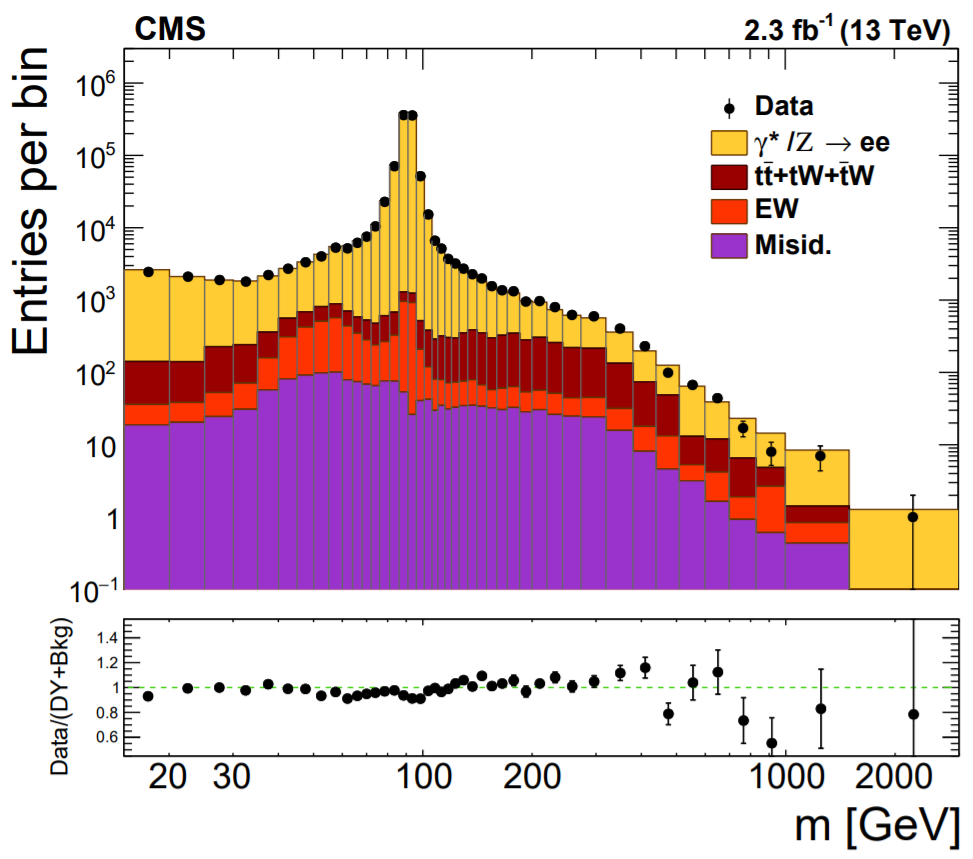
\includegraphics[width=.96\linewidth]{Figure1.png}
	\end{center}
\end{minipage}
\hfill
\begin{minipage}{0.49\textwidth}
	\begin{center}
		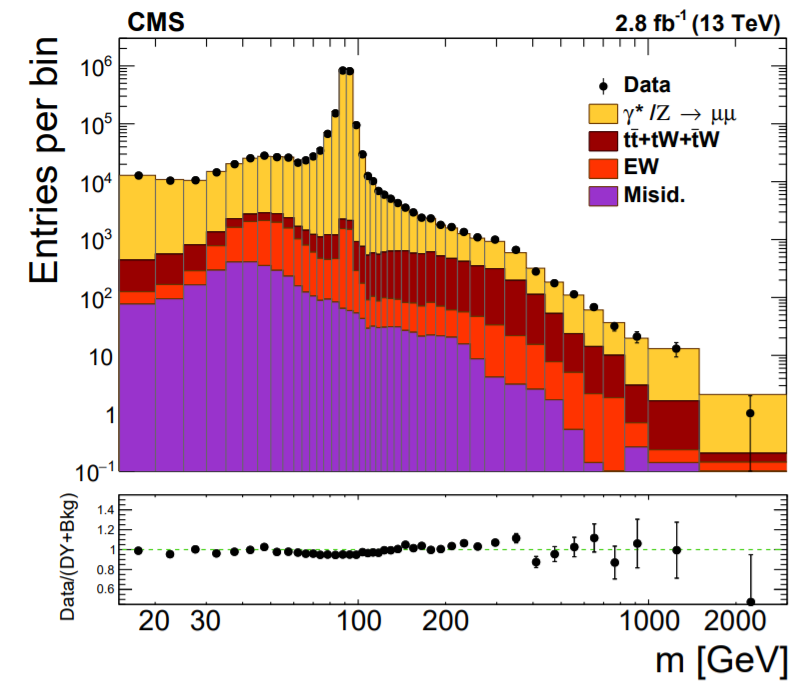
\includegraphics[width=.99\linewidth]{Figure2.png}
	\end{center}
\end{minipage}
\vspace{-0.2cm}
\captionof{figure}{Dielectron (left) and dimuon (right) invariant mass spectra at the proton-proton collision energy of 13 TeV  \cite{DY13}.
      The black dots represent the number of events measured with the CMS detector.
      The colors represent contribution of different processes.
      Yellow color marks the signal -- the Drell-Yan process events.
      ``EW'' denotes diboson and $\mathrm{DY}\rightarrow\tau\tau$ processes.
      ``Misid.'' corresponds to $W+\mathrm{Jets}$ and $QC\!D$ processes.
      The black vertical lines represent statistical uncertainties.}

\vspace{0.3cm}
\begin{thebibliography}{References}

\bibitem{DY13}CMS Collaboration, Measurement of the differential Drell-Yan cross section in proton-proton collisions at $\sqrt{s}=13$ TeV, CMS-SMP-17-001 (2018).

\bibitem{higgs}M.\ B.\ Kiani, Measurement of properties of the Higgs boson decaying to pairs of W and Z bosons at 13 TeV with the
CMS experiment, CMS-CR-2017-267 (2017).

\bibitem{DY8CMS}CMS Collaboration, Measurements of differential and double-differential Drell-Yan cross sections in proton-proton
collisions at $\sqrt{s}=8$ TeV, Eur. Phys. J. C \textbf{75} 147 (2015).

\bibitem{DY8ATLAS}ATLAS Collaboration, Measurement of the triple-differential Drell-Yan cross section in $pp$ collisions at $\sqrt{s}=8$ TeV,
JHEP \textbf{12}, 059 (2017).

\bibitem{DY7}CMS Collaboration, Measurement of the differential and double-differential Drell-Yan cross sections in proton-proton collisions
at $\sqrt{s}=7$ TeV, JHEP \textbf{12}, 030 (2013).

\end{thebibliography}

\end{document}
